\begin{figure}[H]
    \begin{subfigure}{.5\textwidth}
        \centering
        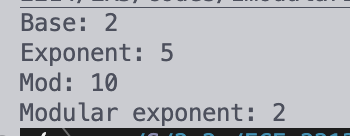
\includegraphics[width=.8\linewidth, height = .73in]{images/output/expo1.png}
        \caption*{}
        \label{fig:expo1}
    \end{subfigure}
    \begin{subfigure}{.5\textwidth}
        \centering
        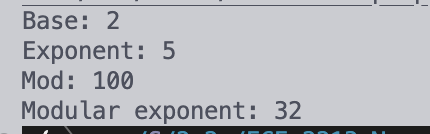
\includegraphics[width=.8\linewidth]{images/output/expo2.png}
        \caption*{}
        \label{fig:expo2}
    \end{subfigure}
    \begin{subfigure}{.5\textwidth}
        \centering
        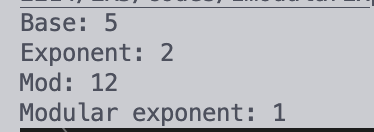
\includegraphics[width=.8\linewidth]{images/output/expo3.png}
        \caption*{}
        \label{fig:expo3}
    \end{subfigure}
    \begin{subfigure}{.5\textwidth}
        \centering
        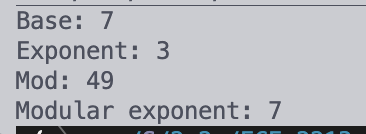
\includegraphics[width=.8\linewidth]{images/output/expo4.png}
        \caption*{}
        \label{fig:expo4}
    \end{subfigure}
    \caption{Outputs for Modular Exponentiation}
    \label{fig:expo}
\end{figure}
\begin{figure}[H]
    \begin{subfigure}{.5\textwidth}
        \centering
        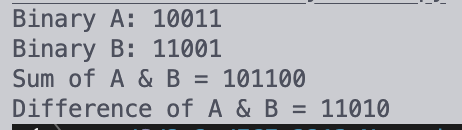
\includegraphics[width=.8\linewidth]{images/output/bin1.png}
        \caption*{}
        \label{fig:bin1}
    \end{subfigure}
    \begin{subfigure}{.5\textwidth}
        \centering
        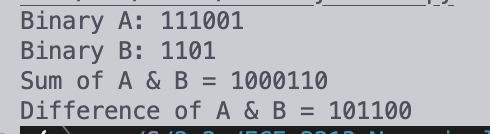
\includegraphics[width=.8\linewidth]{images/output/bin2.png}
        \caption*{}
        \label{fig:bin2}
    \end{subfigure}
    \newline
    \begin{subfigure}{.5\textwidth}
        \centering
        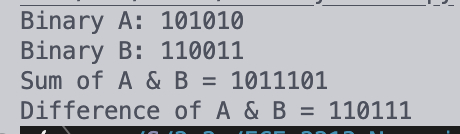
\includegraphics[width=.8\linewidth]{images/output/bin3.png}
        \caption*{}
        \label{fig:bin3}
    \end{subfigure}
    \begin{subfigure}{.5\textwidth}
        \centering
        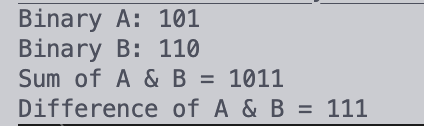
\includegraphics[width=.8\linewidth]{images/output/bin4.png}
        \caption*{}
        \label{fig:bin4}
    \end{subfigure}
    \caption{Outputs for Contraposition}
    \label{fig:bin}
\end{figure}

\begin{figure}[H]
    \begin{subfigure}{.5\textwidth}
        \centering
        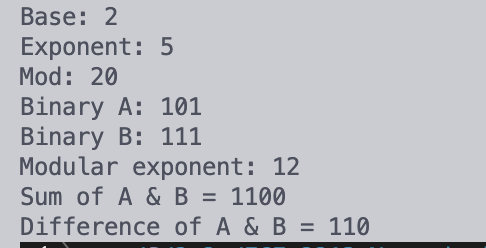
\includegraphics[width=.8\linewidth]{images/output/int1.png}
        \caption*{}
        \label{fig:int1}
    \end{subfigure}
    \begin{subfigure}{.5\textwidth}
        \centering
        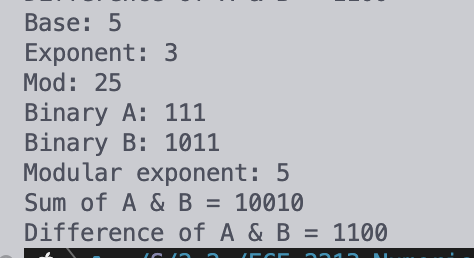
\includegraphics[width=.8\linewidth, height=1.1in]{images/output/int2.png}
        \caption*{}
        \label{fig:int2}
    \end{subfigure}
    \begin{subfigure}{.5\textwidth}
        \centering
        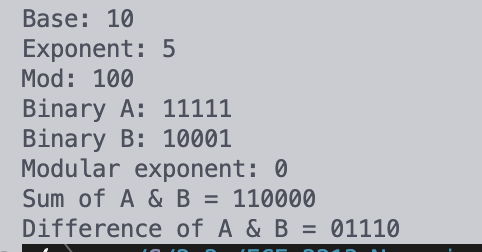
\includegraphics[width=.8\linewidth,]{images/output/int3.png}
        \caption*{}
        \label{fig:int3}
    \end{subfigure}
    \begin{subfigure}{.5\textwidth}
        \centering
        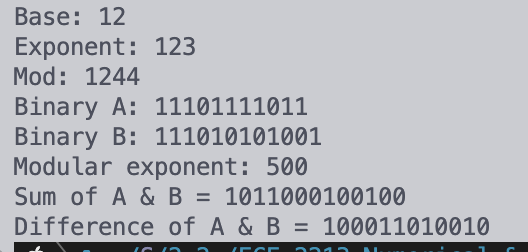
\includegraphics[width=.8\linewidth]{images/output/int4.png}
        \caption*{}
        \label{fig:int4}
    \end{subfigure}
    \caption{Outputs for Logical Equivalence}
    \label{fig:int}
\end{figure}